\documentclass{article}

\usepackage[a4paper]{geometry}
\usepackage[spanish]{babel}
\usepackage{xcolor}

\usepackage{mathbbol}
\usepackage{amsmath}
\usepackage{amsfonts}
\usepackage{hyperref}
\usepackage{graphicx}
\usepackage{subcaption}

\usepackage{algorithm}
\usepackage{algpseudocode}

% Cambiar 'Cuadro' -> 'Tabla'
\addto\captionsspanish{
    \renewcommand{\tablename}{Tabla}
}

\begin{document}

\begin{center}
    {\Large Aprendizaje Automático para Datos en Grafos} \\
    {\LARGE \textbf{Laboratorio 2}} \\
    \vspace{2em}
    \begin{minipage}{0.45\textwidth}
        \centering
        Graciana Castro \\
        4.808.848-2 \\
        gcastro@fing.edu.uy
    \end{minipage}
    \hfill
    \begin{minipage}{0.45\textwidth}
        \centering
        Julian O'Flaherty \\
        6.285.986-9 \\
        julian.o.flaherty@fing.edu.uy
    \end{minipage}
\end{center}


\section{Introducción}


Se presenta a continuación el informe del Laboratorio 2 para la materia Aprendizaje Automático para Datos en Grafos. El objetivo principal de este trabajo es analizar empíricamente propiedades estructurales de grandes redes reales y profundizar en el estudio de algoritmos de partición y detección de comunidades en grafos. A lo largo del laboratorio se busca validar conceptos teóricos vistos en clase, aplicando herramientas como \textit{NetworkX}, \textit{PyTorch Geometric} y \textit{graspologic}, y desarrollar habilidades para la interpretación de resultados obtenidos sobre diferentes tipos de grafos.

En la sección \ref{sec: datasets} del informe se presentan las bases de datos utilizadas en el laboratorio. En el primer ejercicio, presentado en la sección \ref{sec: estructuras}, se estudian propiedades globales y estructura de grandes redes, como la distribución de grados y la modularidad. Se trabaja con las bases de datos de citaciones entre papers y de vuelos entre aeropuertos. En la sección \ref{sec: comunidades} se implementan y comparan algoritmos espectrales para la partición y detección de comunidades en grafos, aplicándolos sobre el grafo de Zachary's Karate Club y sobre un grafo real de blogs políticos.

El código implementado puede consultarse en el repositorio de GitHub \url{https://github.com/j-oflaherty/AA-grafos/blob/main/lab2/Lab2_AAG2025.ipynb}.

\section{Bases de datos utilizadas} \label{sec: datasets}
Para este trabajo se utilizan las siguientes bases de datos:
\begin{itemize}
    \item \textbf{Citations (Cora)}: Esta base de datos contiene información sobre citaciones entre artículos científicos. Cada nodo representa un artículo, y una arista dirigida del nodo A al nodo B indica que el artículo A cita al artículo B. Es un grafo no dirigido que contiene 2708 nodos y 10556 aristas.
    \item \textbf{Airports}: Esta base de datos contiene información sobre vuelos entre aeropuertos. Cada nodo representa un aeropuerto, y una arista dirigida del nodo A al nodo B indica que existe un vuelo directo desde el aeropuerto A al aeropuerto B. Es un grafo dirigido que contiene 1190 nodos y 13599 aristas.
    \item \textbf{Zachary's Karate Club}: Presentada en el laboratorio anterior, esta base de datos representa las interacciones sociales entre los miembros de un club de karate. Cada nodo representa a un miembro del club, y una arista entre dos nodos indica que esos miembros interactúan socialmente.
    \item \textbf{Political Blogs}: Esta base de datos contiene información sobre blogs políticos y las conexiones entre ellos. Cada nodo representa un blog, y una arista entre dos nodos indica que el blog del que sale la arista tiene un link al blog al que llega la arista. Para el laboratorio se trabajará con la versión no dirigida, que tiene una arista entre dos nodos si existe una arista en cualquiera de los sentidos. Este grafo tiene 1490 nodos y 19025 aristas.
\end{itemize}


\section{Estructuras de grandes redes} \label{sec: estructuras}

\subsection{Distribución de grados}

La distribución de grados de un grafo $G$ se refiere al conjunto de fracciones $p_k$ que representan la proporción de vértices con grado $k$ en el grafo. Es una medida importante para caracterizar la estructura de la red, ya que proporciona información sobre cómo se conectan los nodos entre sí.


En muchas redes reales, como las redes sociales o las redes de citas académicas, la distribución de grados sigue una \textit{power-law}, que se define de la forma: $p_k = Ck^{-\alpha}$, donde $C$ es una constante de normalización y $\alpha$ es el exponente que caracteriza la distribución. Esta forma implica que la probabilidad de encontrar un nodo con grado $k$ disminuye rápidamente a medida que $k$ aumenta.


\textcolor{red}{En la figura \ref{fig: degree_distribution} se muestra la distribución de grados del grafo de citaciones entre papers. Se observa que existe un rango de $k$ para el cual la distribución sigue una \textit{power-law}; sin embargo, no se cumple para todos los valores (hecho que no resulta extraño en redes reales). Para evidenciar si efectivamente la distribución sigue una \textit{power-law} en cierto rango, se realiza la gráfica utilizando \textit{bins} equiespaciados, donde la tendencia lineal se hace más evidente.}

\textcolor{blue}{En la figura \ref{fig: degree_distribution} se muestra la distribución de grados del grafo de citaciones entre papers. En la figura \ref{fig: degree_distribution_lineal} se observa la distribución en bins equiespaciados donde se puede observar la tendencia lineal, aunque contiene muchos bins que no se ajustan a esa distribución. Esto sucede por la falta de datos, a medida que aumenta el grado hay menos nodos, por lo que los bins tienen menos muestras. Para contrarestar este efecto, se eligen bins en escala logarítmica con base 2, donde en la figura~\ref{fig: degree_distribution_log} se puede observar la tendencia lineal en el rango de $k$ para el cual la distribución sigue una \textit{power-law}.}

\begin{figure}
    \centering
    \begin{subfigure}[b]{0.48\textwidth}
        \centering
        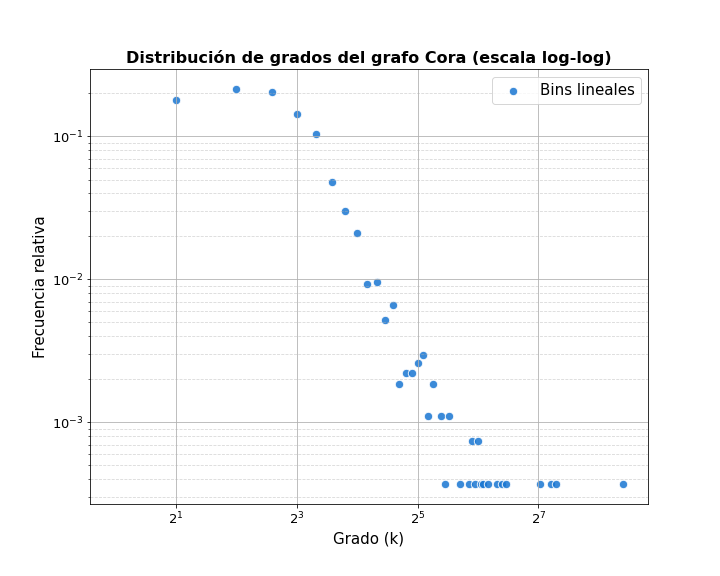
\includegraphics[width=\textwidth]{imagenes/dist_grado_Cora_lineal.png}
        \caption{Distribución de grados en bins equiespaciados}
        \label{fig: degree_distribution_lineal}
    \end{subfigure}
    \hfill
    \begin{subfigure}[b]{0.48\textwidth}
        \centering
        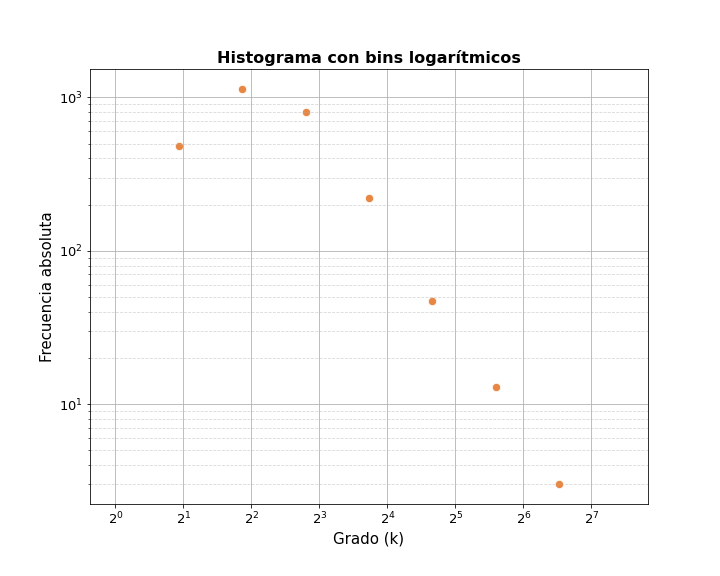
\includegraphics[width=\textwidth]{imagenes/dist_grado_Cora_log.png}
        \caption{Distribución de grados en escala logarítmica}
        \label{fig: degree_distribution_log}
    \end{subfigure}
    \caption{Distribución de grados del grafo de citaciones entre papers. En la figura \ref{fig: degree_distribution_lineal} se muestra en bins equiespaciados, mientras que en la figura \ref{fig: degree_distribution_log} se observa la distribución en escala logarítmica.}
    \label{fig: degree_distribution}
\end{figure}


La distribución que se observa en la figura \ref{fig: degree_distribution_log} sigue la denominada \textit{Distribución de Pareto}. Una variable aleatoria $X$ se dice que tiene distribución de Pareto si tiene una función de densidad de probabilidad dada por:

\begin{equation}
    \label{eq:pareto}
    p(k) = \left\lbrace \begin{array}{c c} C k^{-\alpha} & \text{ si } k\geq k_\text{min} \\ 0 & \text{ en otro caso} \end{array}\right.
\end{equation}


Para hallar el $C$ que verifica que esta distribución es una densidad, se integra sobre su dominio y se iguala a 1:

$$
    \int_{0}^{\infty} p(k) dk = \int_{k_{\text{min}}}^{\infty} C k^{-\alpha} dk = C \int_{k_{\text{min}}}^{\infty} k^{-\alpha}dk \\
    \int_{0}^{\infty} p(k) dk = C \left[ \frac{k_{\text{min}}^{-\alpha+1}}{-\alpha+1} \right] = 1 \\
    \Rightarrow C = \frac{-\alpha+1}{k_{\text{min}}^{-\alpha+1}}
$$


Como se demuestra en la sección \ref{sec: pareto}, el estimador de máxima verosimilitud para el exponente $\alpha$ de la distribución de Pareto es:

\begin{equation}
    \label{eq: alpha_pareto}
    \hat{\alpha} = 1 + n \left[ \sum_{i=1}^{n} \ln\left(\frac{k_i}{k_{\text{min}}}\right) \right]^{-1}
\end{equation}

Para calcularlo, se implementa una función que recibe como parámetros una lista de los grados de un grafo y el valor de $k$ a partir del cual vale la \textit{power-law}. Aplicando esta función al grafo de citaciones entre papers, considerando $k_{\text{min}} = 10$, se obtiene un valor de $\hat{\alpha} = 4.030$.

\subsection{Assortative Mixing}

Se define el \textit{assortative mixing} como la tendencia de los nodos en una red a conectarse con otros nodos que son similares en algún aspecto. En el contexto de redes sociales, por ejemplo, esto puede significar que las personas tienden a formar conexiones con otras personas que tienen intereses, antecedentes o características demográficas similares. Se utiliza como medida de similaridad la \textit{modularidad}, que mide la proporción entre las aristas que hay entre nodos de un mismo tipo y las esperadas si la asignación de aristas fuera aleatoria. Formalmente, está definida como:

\begin{equation}
    \label{eq: modularity}
    Q = \frac{1}{2m} \sum_{ij} \left(A_{ij} -\frac{k_ik_j}{2m} \right)\delta(c_i,c_j)
\end{equation}

donde $m$ es la cantidad total de aristas en la red, $A_{ij}$ son las entradas de la matriz de adyacencia, $k_i$ es el grado del nodo $i$ y $\delta(r,p)$ es la delta de Kronecker: $\delta(r,p) = 1$ si $r=p$ y $\delta(r,p) = 0$ si $r\neq p$. Toma valores mayores a uno si hay mucha interconexión entre nodos del mismo tipo, y valores menores a uno en el caso contrario.


Para el cálculo de modularidad, se utiliza primero una función que recibe las etiquetas del grafo para separarlo en comunidades y luego calcula la modularidad utilizando la función \verb|networkx.algorithms.community.modularity|. Se obtienen los siguientes resultados para las bases de datos de citaciones entre papers y de vuelos entre aeropuertos:
\begin{itemize}
    \item \textbf{Citations (Cora)}: La modularidad obtenida es $Q = 0.640$.
    \item \textbf{Airports}: La modularidad obtenida es $Q = 0.108$.
\end{itemize}

Se entiende que es coherente que la modularidad del grafo de aeropuertos sea baja, ya que los aeropuertos poco transitados suelen tener vuelos hacia aeropuertos más grandes, y no entre ellos. La modularidad del grafo de citaciones es más alta, ya que los artículos tienden a citar otros artículos relacionados a la misma disciplina.

\section{Detección de comunidades} \label{sec: comunidades}

En esta sección trabajaremos sobre el grafo de Zachary's Karate Club, un grafo muy conocido por ser un desafío para la detección de comunidades aunque es un grafo pequeño. El grafo surge del análisis de las interacciones sociales entre miembros de un club de karate, y como quedo divido  el club luego de su disolución.

\begin{figure}[htb]
    \centering
    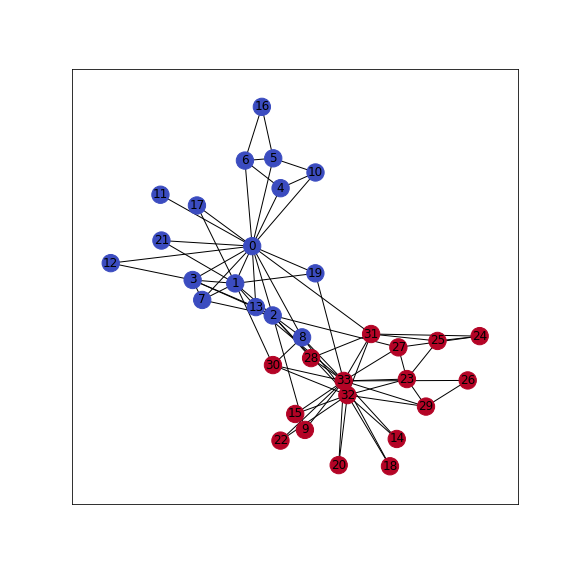
\includegraphics[width=0.8\textwidth]{imagenes/karate_club.png}
    \caption{Grafo de Zachary's Karate Club. El color del nodo indica la comunidad a la que pertenece.}
    \label{fig: karate_club}
\end{figure}

Nuestro objetivo cuando hacemos análisis de comunidades es encontrar la partición del grafo observada en figura~\ref{fig: karate_club} solo a partir de las relaciones entre los nodos. Los métodos se pueden dividir en dos categorías:
\begin{itemize}
    \item \textbf{Partición de grafo}: Busca dividir el grafo en dos comunidades de tamaño fijo, que es un parámetro modificable del algoritmo.
    \item \textbf{Detección de comunidades}: Busca encontrar comunidades en el grafo sin pre-especificar el tamaño.
\end{itemize}

\subsection{Spectral Partitioning}

El \emph{Spectral Clustering} es un método de partición de grafos que se basa en la descomposición espectral de la matriz de adyacencia. El algoritmo busca hacer la partición del grafo que minimiza el costo del corte, donde el costo se define como la cantidad de aristas que se cortan. Matemáticamente, queremos hallar $\mathbf{s}\in{\pm 1}^{N_v}$ que minimice el costo del corte:
\begin{equation*}
    C = \frac{1}{2} \sum_{i,j} A_{ij} (1 - \mathbf{s}_i \mathbf{s}_j)
\end{equation*}
Relajando $\mathbf{s}\in{\pm 1}^{N_v}$ a $\mathbf{\hat{s}}\in{\mathbb{R}}^{N_v}$, podemos plantear el problema como:
\begin{equation*}
    \mathbf{\hat{s}} = \arg \min_{\mathbf{s}\in{\mathbb{R}}^{N_v}} \mathbf{s}^\top \mathbf{L} \mathbf{s}, \quad \text{sujeto a } \mathbf{1}^\top \mathbf{s} = N_1 - N_2 \text{ y } \mathbf{s}^\top \mathbf{s} = 1
\end{equation*}
Fiedler~\cite{Fiedler1973} caracterizó este problema y demostró que la solución es:
\begin{equation*}
    \mathbf{\hat{s}} = \mathbf{v}_2 + \frac{N_1 - N_2}{N_v} \mathbf{1}
\end{equation*}
donde $\mathbf{v}_2$ es el vector asociado al segundo valor propio más chico de la matriz Laplaciana $\mathbf{L}$, al que se le da el nombre de vector de \emph{Fiedler}. Para asignar las
etiquetas de las comunidades, maximizamos la similitud $\mathbf{s}^\top\mathbf{\hat{s}}$, lo que resulta en
\begin{equation}
    \label{eq: fiedler_asignation}
    s_i = f(\mathbf{v}_2) = \left\lbrace 
    \begin{array}{c l}
         1, & \text{si } [\mathbf{v}_2]_i \text{ esta entre las $N_1$ componentes más grandes de $\mathbf{v}_2$} \\
        -1, & \text{en otro caso}
    \end{array}\right.
\end{equation}
El pseudocódigo de \emph{Spectral Partitioning} se describe en el algoritmo~\ref{alg: spectral_partitioning}.
\begin{algorithm}
    \caption{Spectral Partitioning}
    \label{alg: spectral_partitioning}
    \begin{algorithmic}
    \Require Grafo $G = (V, E)$ con $n$ nodos; $n_1$, $n_2$ enteros positivos tales que $n_1 + n_2 = n$
    \State  $\mathbf{L} \leftarrow $ laplaciana de G
    \State $\mathbf{v}_2 \leftarrow $ vector asociado al segundo valor propio más chico de $\mathbf{L}$ (vector de Fiedler)\\ 
    \Return $\mathbf{s} = \mathbf{f}(\mathbf{v}_2)$ con $\mathbf{f}=(f_1,f_2,\ldots,f_N)$ y $f$ definida en \eqref{eq: fiedler_asignation}
    \end{algorithmic}
\end{algorithm}

En la figura \ref{fig: spectral_partitioning} se puede observar la partición del grafo de Zachary's Karate Club utilizando el algoritmo de Spectral Partitioning con $n_1 = n_2 = 17$. Se observa que el algoritmo divide perfectamente el grafo, descubriendo las comunidades correctas.

\begin{figure}[htb]
    \centering
    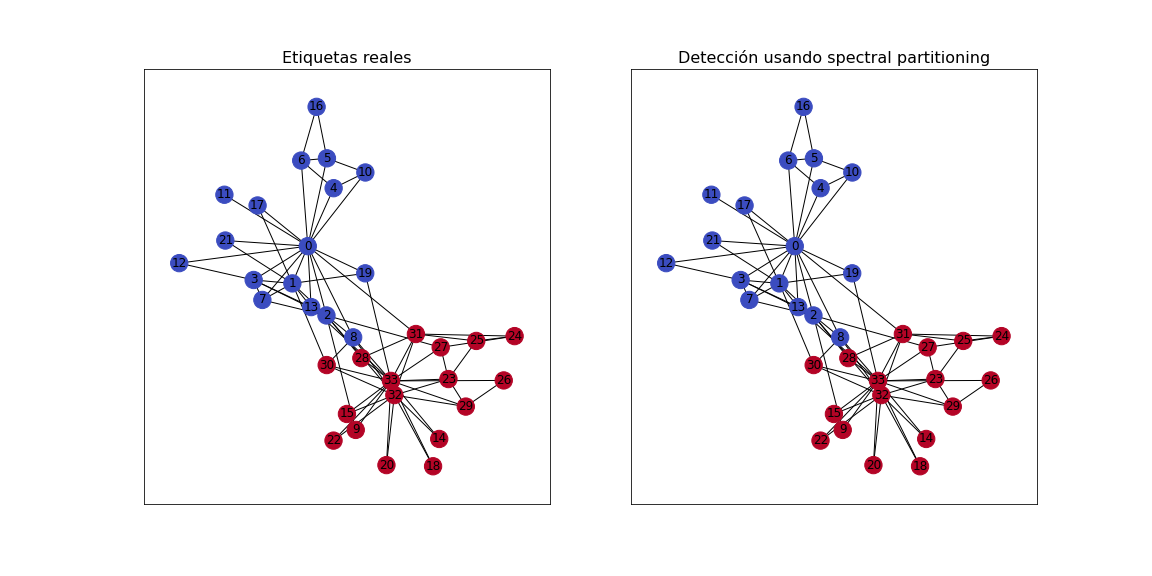
\includegraphics[width=\textwidth]{imagenes/spectral_partitioning.png}
    \caption{Partición del grafo de Zachary's Karate Club utilizando el algoritmo de Spectral Partitioning.}
    \label{fig: spectral_partitioning}
\end{figure}

\subsection{Evaluación de la partición}

\subsubsection{Índice de Rand}

Además de una evaluación visual, podemos usar una métrica como el índice de Rand, que evalúa la similitud de clusters de datos. Dado un conjunto de $n$ elementos $S$, y dos particiones $X = {X_1, X_2, \ldots, X_k}$ e $Y = {Y_1, Y_2, \ldots, Y_l}$, el índice de Rand ajustado se define como:
\begin{equation*}
    R = \frac{a + b}{a + b + c + d} = \frac{a + b}{\binom{n}{2}}
\end{equation*}
donde:
\begin{itemize}
    \item $a$ es el número de pares de elementos que están en el mismo cluster en $X$ y en $Y$.
    \item $b$ es el número de pares de elementos que están en diferentes clusters en $X$ y en $Y$.
    \item $c$ es el número de pares de elementos que están en el mismo cluster en $X$ y en diferentes clusters en $Y$.
    \item $d$ es el número de pares de elementos que están en diferentes clusters en $X$ y en el mismo cluster en $Y$.
\end{itemize}
Idealmente, este indice debería ser 0 si la particiones son aleatorias, y 1 si son idénticas. El problema, es que con la formulación presentada anteriormente, en particiones aleatorias va a suceder que haya pares que esten en el mismo cluster en $X$ e $Y$, por lo que se introduce el índice de Rand corregido como una medida más robusta. 

El índice de Rand ajustado (ARI) se define como:
\begin{equation}
    ARI = \frac{\sum_{ij} \binom{n_{ij}}{2} - \left[\sum_i \binom{n_{i\cdot}}{2} \sum_j \binom{n_{\cdot j}}{2}\right] / \binom{n}{2}}{\frac{1}{2}\left[\sum_i \binom{n_{i\cdot}}{2} + \sum_j \binom{n_{\cdot j}}{2}\right] - \left[\sum_i \binom{n_{i\cdot}}{2} \sum_j \binom{n_{\cdot j}}{2}\right] / \binom{n}{2}}
\end{equation}
donde $n_{ij}$ es el número de elementos que están en el cluster $i$ de la partición $X$ y en el cluster $j$ de la partición $Y$, $n_{i\cdot} = \sum_j n_{ij}$ es el número total de elementos en el cluster $i$ de $X$, y $n_{\cdot j} = \sum_i n_{ij}$ es el número total de elementos en el cluster $j$ de $Y$.

Para el grafo de Zachary's Karate Club particionado con Spectral Partitioning, se obtiene un ARI de $1.00$. Si corremos el índice sobre una partición al azar, se obtiene un ARI de $0.00$.

\subsection{Indice de Fowkles-Mallows}

El índice de Fowkles-Mallows (FM) es la media geómetrica de la precisión y el recall del clustering. Matemáticamente, se define como:
\begin{equation}
    FM = \sqrt{\frac{a}{a+c}\frac{b}{b+d}}
\end{equation}
usando las definiciones de $a$, $b$, $c$ y $d$ de la sección anterior. El valor mínimo del índice es 0 y el valor máximo es 1, que se obtiene cuando las particiones son idénticas. 

Para el grafo de Zachary's Karate Club particionado con Spectral Partitioning, también se obtiene un FM de $1.00$, pero a diferencia del ARI, si lo corremos sobre una partición al azar, se obtiene un FM de $0.696$. Por lo que concluímos que el spectral partitioning es un buen método para particionar el grafo de Zachary's Karate Club, teniendo la información a priori del tamaño de las comunidades.

\subsection{Partición por espectro modularidad máxima}

Observamos que el \emph{Spectral Partitioning} obtiene un resultado perfecto en el grafo, pero este método tiene la limitante que require el tamaño de las comunidades para hacer el clustering. Esto límita mucho la utilidad, dado que en general no se sabe el tamaño de las comunidades a priori.

Existen métodos que no tienen esa limitante, cómo el método de \emph{Spectral Modularity Maximization}. En el método anterior, buscabamos la partición que minimizaba el costo del corte. En este método, vamos a buscar la partición que maximiza la modularidad~\eqref{eq: modularity}. Al igual que en el método anterior, definimos el vector $\mathbf{s}\in{\pm 1}^{N_v}$, donde un $1$ indica pertenecer a la comunidad 1 y un $-1$ indica pertenecer a la comunidad 2. Por lo que podemos escribir el problema como:
\begin{equation*}
    Q(G, S) = \frac{1}{2N_e} \sum_{i,j\in V}\left[A_{ij} - \frac{k_i k_j}{2N_e}\right] \frac{1}{2}(s_is_j + 1) \\
\end{equation*}
Definiendo $B_{ij} = A_{ij} - \frac{k_i k_j}{2N_e}$, podemos reescribir el problema como:
\begin{equation*}
    Q(G, S) = \frac{1}{4N_e} \sum_{i,j\in V}B_{ij}(s_is_j + 1) \stackrel{\sum_jB_{ij} = 0}{=} \frac{1}{4N_e} \sum_{i,j\in V}B_{ij}s_is_j = \frac{1}{4N_e} \mathbf{s}^\top \mathbf{B} \mathbf{s}
\end{equation*}
Al igual que en el problema anterior, optimizar $\mathbf{s}$ directamente es un problema NP-hard, por lo que se relaja el problema de optimización optimizando $\mathbf{\hat{s}} \in \mathbb{R}^{N_v}$ en lugar de $\mathbf{s}$, con $||\mathbf{s}||_2 = \sqrt{N_v}$.
Por lo que el problema de optimización resultante es
\begin{equation*}
    \mathbf{\hat{s}} = \arg \max_{\mathbf{s}\in{\mathbb{R}}^{N_v}} \mathbf{s}^\top \mathbf{B} \mathbf{s}, \quad \text{sujeto a } \mathbf{s}^\top \mathbf{s} = N_v
\end{equation*}
La solución a este problema es:
\begin{equation*}
    \mathbf{\hat{s}} = \mathbf{v}_2
\end{equation*}
donde $\mathbf{v}_2$ es el vector asociado al segundo valor propio más grande de la matriz $B$. Aplicando multiplicadores de Lagrange y despejando, llegamos a:
\begin{equation*}
    \mathbf{B}\mathbf{s} = \lambda \mathbf{s}
\end{equation*}
Por lo que $\mathbf{s}$ es un vector propio de $\mathbf{B}$ con valor propio $\lambda$. Cómo estamos buscando máximizar $\mathbf{s}^\top \mathbf{B} \mathbf{s} = \lambda$, nos interesa el vector propio dominante $\mathbf{u}_1$ de $\mathbf{B}$. Por último, para obtener la asignación de comunidades, máximizamos $\mathbf{s}^\top \mathbf{u}_1$, lo que resulta en:
\begin{equation*}
    s_i = \text{signo}([\mathbf{u}_1]_i) = \left\lbrace 
    \begin{array}{c l}
         1, & \text{si } [\mathbf{u}_1]_i > 0 \\
        -1, & \text{si } [\mathbf{u}_1]_i \leq 0
    \end{array}\right.
\end{equation*}
Podemos resumir el método como el procedimiento descrito en el algoritmo~\ref{alg: spectral_modularity_maximization}.
\begin{algorithm}
    \caption{Spectral Modularity Maximization}
    \label{alg: spectral_modularity_maximization}
    \begin{algorithmic}
    \Require Grafo $G = (V, E)$ con $n$ nodos y $N_e$ aristas
    \State $\mathbf{B} \leftarrow $ matriz de modularidad de G ($\mathbf{B}_{ij} = A_{ij} - \frac{k_i k_j}{2N_e}$)
    \State $\mathbf{u}_1 \leftarrow $ vector propio dominante de $\mathbf{B}$ \\ 
    \Return $\mathbf{s} = \text{signo}(\mathbf{u}_1)$
    \end{algorithmic}
\end{algorithm}


Aplicando el método en el grafo de Zachary's Karate Club, obtenemos las comunidades mostradas en la figura \ref{fig: spectral_modularity_maximization}. A método anterior, en este método encontramos que el nodo 8 fue mal clasificado, siendo asignado a una comunidad incorrecta. Para esta partición, obtenemos un ARI de $0.882$ y un FM de $0.939$.

\begin{figure}[htb]
    \centering
    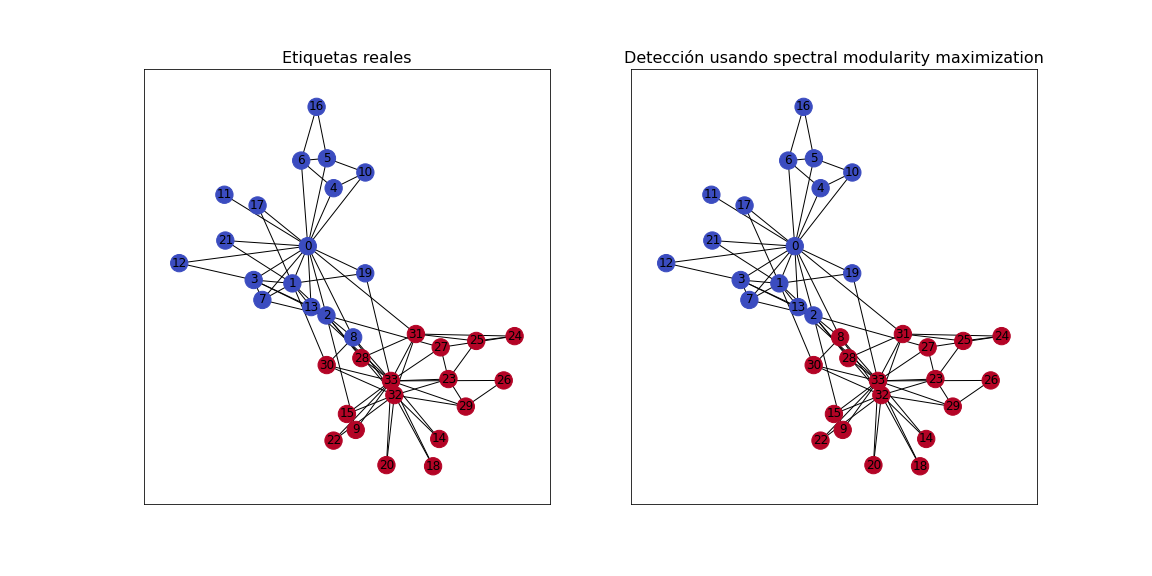
\includegraphics[width=\textwidth]{imagenes/spectral_modularity_maximization.png}
    \caption{Partición del grafo de Zachary's Karate Club utilizando el algoritmo de Spectral Modularity Maximization.}

    \label{fig: spectral_modularity_maximization}
\end{figure}




\section{Estimador de máxima verosimilitud para el exponente de la distribución de Pareto} \label{sec: pareto}

Sea $X$ una variable aleatoria con distribución de Pareto, por lo tanto su función de densidad de probabilidad es:

$$p(x) = \left\lbrace \begin{array}{c c} C x^{-\alpha} & \text{ si } x\geq x_\text{min} \\ 0 & \text{ en otro caso} \end{array}\right.$$

\subsection{Función de log-verosimilitud}

La función de log-verosimilitud para una muestra $x_1, x_2, \ldots, x_n$ es la suma de los logaritmos de las funciones de densidad evaluadas en cada punto de la muestra. Para el ejercicio presentado en la sección \ref{sec: estructuras}, en que se tiene una Distribución de Pareto con $C = \frac{-\alpha+1}{k_{\text{min}}^{-\alpha+1}}$, se halla la función de log-verosimilitud:

\begin{align}
    \mathcal{L}_n(\alpha) & = \log \left[\prod_{i=1}^{n} \left( \frac{1-\alpha}{k_{\text{min}}^{1-\alpha}} k_i^{-\alpha} \right) \right] \nonumber               \\
                          & = \sum_{i=1}^{n} \left[ \log(1-\alpha) - log\log(k_{\text{min}}) - \log \left(\frac{k_i}{k_{min}} \right)^{\alpha} \right] \nonumber \\
                          & = n \log(1-\alpha) - n\log(k_{\text{min}}) - \alpha \sum_{i=1}^{n} \log\left(\frac{k_i}{k_{min}} \right)
\end{align}

donde en la primera igualdad se toma el logaritmo, en la segunda se utiliza la propiedad de que el logaritmo del producto es la suma de los logaritmos, y en la tercera se resuelven las sumatorias que no dependen de $i$ y se utiliza la propiedad del logaritmo de la potencia.

\subsection{Estimador de Máxima Verosimilitud para $\alpha$}

Partiendo de la ecuación \ref{eq: log-verosimilitud}, se deriva respecto a $\alpha$ e iguala a cero para encontrar el máximo:
$$
    \frac{d\mathcal{L}_n(\alpha)}{d\alpha} = \frac{n}{\alpha -1} - \sum_{i=1}^n \log \left(\frac{k_i}{k_\text{min}}\right) = 0 \\
    \Rightarrow \frac{n}{\alpha -1} = \sum_{i=1}^n \log \left(\frac{k_i}{k_\text{min}}\right) \\
    \Rightarrow \hat{\alpha} = 1 + n \left[ \sum_{i=1}^{n} \ln\left(\frac{k_i}{k_\text{min}}\right) \right]^{-1}
$$

\section{Referencias}
\bibliographystyle{plain}
\bibliography{refs}

\end{document}